
\documentclass{standalone}
\usepackage[svgnames]{xcolor}
\usepackage{pgfplots}
\pgfplotsset{compat=newest}
\usepackage[sfdefault]{FiraSans}
\usepackage{FiraMono}
\renewcommand*\familydefault{\sfdefault}
\begin{document}
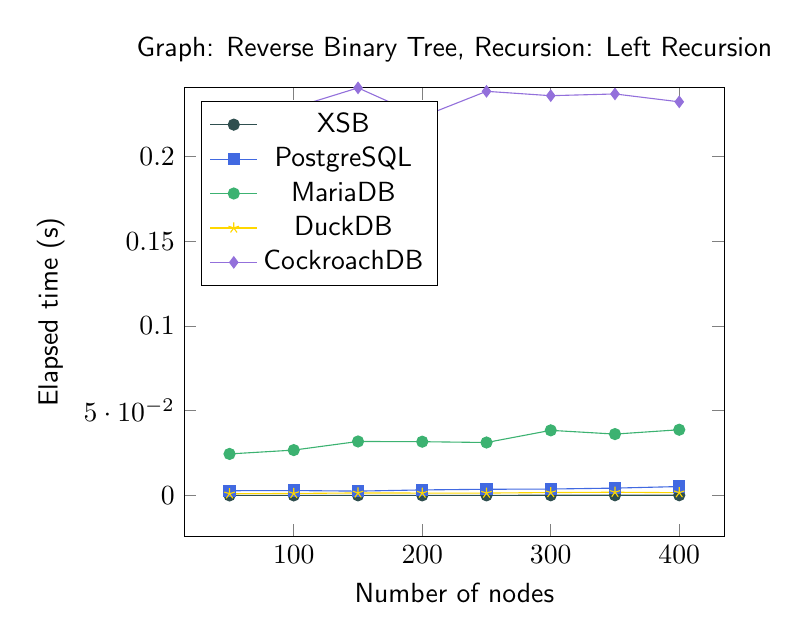
\begin{tikzpicture}
    \begin{axis}[
        title={Graph: Reverse Binary Tree, Recursion: Left Recursion},
        xlabel={Number of nodes},
        ylabel={Elapsed time (s)},
        legend pos={north west},
        ymax=0.24035587498219685
    ]
    \addplot+[DarkSlateGray, mark options={color=DarkSlateGray}] coordinates {(50,2.121925354003906e-05) (100,3.5285949707031236e-05) (150,6.513595581054691e-05) (200,6.432533264160158e-05) (250,6.456375122070314e-05) (300,0.00013866424560546878) (350,0.00013551712036132817) (400,0.0001399993896484376)};
\addlegendentry{XSB}
\addplot+[RoyalBlue, mark options={color=RoyalBlue}] coordinates {(50,0.0028013833914883437) (100,0.0028965249890461563) (150,0.002571641595568508) (200,0.0032741168048232793) (250,0.0036583249806426466) (300,0.003799133002758026) (350,0.004343241616152227) (400,0.005265341186895966)};
\addlegendentry{PostgreSQL}
\addplot+[MediumSeaGreen, mark options={color=MediumSeaGreen}] coordinates {(50,0.024496149993501602) (100,0.026764133619144558) (150,0.03184296699473634) (200,0.031710300187114626) (250,0.03123087522108108) (300,0.03840608317404985) (350,0.03620174978859723) (400,0.038761708198580894)};
\addlegendentry{MariaDB}
\addplot+[Gold, mark options={color=Gold}] coordinates {(50,0.00102458338951692) (100,0.001186941412743181) (150,0.0014917833963409067) (200,0.001413275010418147) (250,0.001425466185901314) (300,0.0017252084100618959) (350,0.0019103166181594134) (400,0.0016389084048569202)};
\addlegendentry{DuckDB}
\addplot+[MediumPurple, mark options={color=MediumPurple}] coordinates {(50,0.22627291680546477) (100,0.22864510818617417) (150,0.24035587498219685) (200,0.22334320819936693) (250,0.23832136678975074) (300,0.2357423918088898) (350,0.2367704498115927) (400,0.23212246680632234)};
\addlegendentry{CockroachDB}

    \end{axis}
\end{tikzpicture}
\end{document}
